\subsection{理論値との比較}
通常の球形粒子にbotton heavy性を仮定した場合について理論値との比較を行う.
この場合,\ref{sec:rotation}で述べたように,粒子にかかるトルクは,式\eqref{eq:sum_of_torque_z}のように表される.
    \begin{align}
        N_z &= \boldsymbol{N}^\mathrm{H}_z + \boldsymbol{N}^\mathrm{b.h.}_z \notag \\
            &= 4 \pi \mu a^3 \dot{\gamma} - \frac{4}{3} \pi a^3 \rho h g \sin \theta
        \tag{\ref{eq:sum_of_torque_z}}
    \end{align}
\noindent
このトルクはFig.\ref{fig:sum_of_torque}のように表される.
ただし,本研究では,粒子の重心と球の中心のずれを$h = 2.5 \Delta$,重力の大きさを$g = 0.06$と設定した.
    \begin{figure}[H]
        \centering
        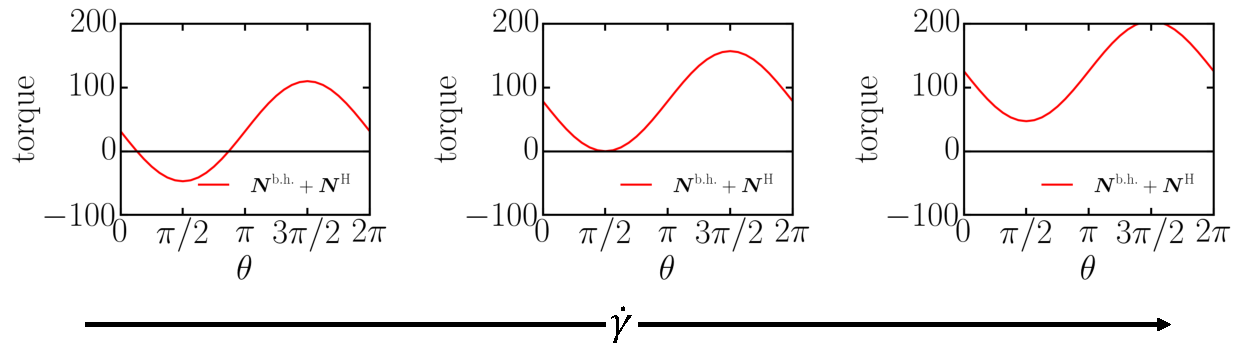
\includegraphics[scale=0.8]{/Users/taiga/Projects/lab/thesis/components/chapter4/figs/sum_of_torque.pdf}
        \caption{流体から受けるトルクとbottom heavy性によるトルクの和.
        黒線は$N_z = 0$を表す.
        (a)$\dot{\gamma} = 0.04$
        (b)$\dot{\gamma} = 0.05$
        (c)$\dot{\gamma} = 0.06$}
        \label{fig:sum_of_torque}
    \end{figure}
\noindent
Fig.\ref{fig:extracted_results}は,Fig.\ref{fig:results}の上段のシミュレーション結果を抜粋したものである.
    \begin{figure}[H]
        \centering
        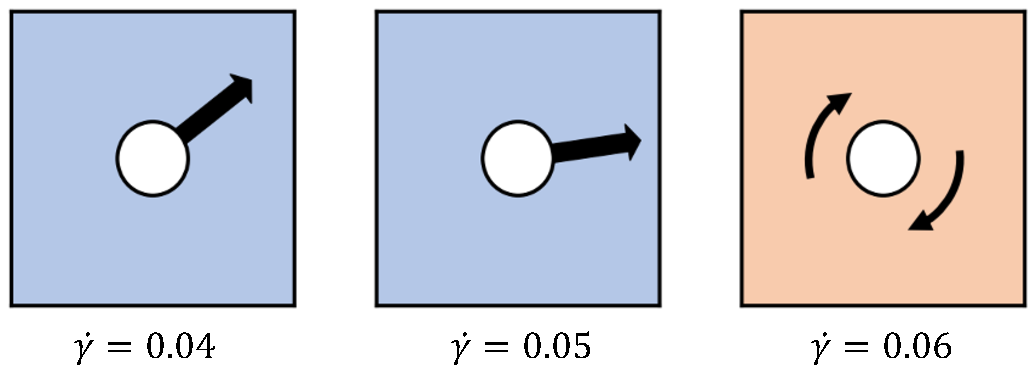
\includegraphics[scale=0.8]{/Users/taiga/Projects/lab/thesis/components/chapter4/figs/extracted_results.pdf}
        \caption{$B_2 = 0$の場合のシミュレーション模式図とそのときのせん断速度の値}
        \label{fig:extracted_results}
    \end{figure}
\noindent
ここで,\ref{sec:condition}で記したパラメータの値と共に,
トルクの計算に必要なパラメータの値を表\ref{tab:parameters}に示す.
    \begin{table}[H]
        \centering
        \caption{シミュレーションで設定したパラメータ}
        \label{tab:parameters}
        \begin{tabular}{cc}
            \hline
            項目 & 値 \\
            \hline
            $a$    & $5$ \\
            $h$    & $2.5$ \\
            $\rho$ & $1.0$ \\
            $\mu$  & $1.0$ \\
            $g$    & $0.06$ \\
            \hline
        \end{tabular}
    \end{table}
これらの値を式\eqref{eq:const_gammadot}に代入し,$\dot{\gamma}_c$を求めると,
    \begin{align}
        \dot{\gamma}_c
        &= \frac{1.0 \cdot 2.5 \cdot 0.06}{3 \cdot 1.0} \\
        &= 0.05
    \end{align}
と求まる.
したがって,$\dot{\gamma} = 0.05$の時,
粒子の進行方向が$\theta = \pi / 2$に固定され,粒子は回転しないと予想される.
$\dot{\gamma} = 0.05$の時のシミュレーション結果では,粒子の進行方向は,
    \begin{equation}
        \theta = 1.4287
    \end{equation}
であった.その相対誤差は0.09であり,概ね一致していると考えられる.
また,$\dot{\gamma} = 0.04$とした場合は,
$N_z = 0$となる角度$\theta$は以下のように予想される.
    \begin{align}
        0 &= 4 \pi \cdot \mu \cdot a^3 \cdot 0.04 - \frac{4}{3} \pi \cdot a^3 \cdot \rho h g \sin{\theta} \\
        \therefore
        \theta
        &= \arcsin{\left( \frac{4 \cdot \pi \cdot 1.0 \cdot 5^3 \cdot 0.04}{4/3 \cdot \pi \cdot 5^3 \cdot 1.0 \cdot 2.5 \cdot 0.06} \right)} \\
        &= 0.9273
    \end{align}
$\dot{\gamma} = 0.04$としたシミュレーション結果はでは,粒子の進行方向は
    \begin{equation}
        \theta = 0.9177
    \end{equation}
であった.その相対誤差は0.01であり,よく一致していることが分かる.
また,$\dot{\gamma} > 0.05$では粒子は定常的に回転すると考えられるが,
シミュレーション結果はそれに反していないことが分かる.
